\documentclass[11pt,a4paper]{article}

% ── Packages ──────────────────────────────────────────────────────────────
\usepackage[utf8]{inputenc}
\usepackage[T1]{fontenc}
\usepackage{lmodern}
\usepackage[margin=1in]{geometry}
\usepackage{hyperref}
\usepackage{xcolor}
\usepackage{booktabs}
\usepackage{array}
\usepackage{enumitem}
\usepackage{amsmath,amssymb}
\usepackage{parskip}
\usepackage{fancyhdr}
\usepackage{float}
\usepackage{graphicx}

% ── Colors ────────────────────────────────────────────────────────────────
\definecolor{purpleballoon}{HTML}{A855F7}
\definecolor{tealballoon}{HTML}{14B8A6}
\definecolor{orangeballoon}{HTML}{F97316}

% ── Hyperref setup ────────────────────────────────────────────────────────
\hypersetup{
    colorlinks=true,
    linkcolor=blue!60!black,
    urlcolor=blue!60!black,
    citecolor=blue!60!black,
}

% ── Header / Footer ──────────────────────────────────────────────────────
\pagestyle{fancy}
\fancyhf{}
\fancyhead[L]{\small BART Scoring Update --- v2 (EV-Based Overhaul)}
\fancyhead[R]{\small\thepage}
\renewcommand{\headrulewidth}{0.4pt}

% ── Title ─────────────────────────────────────────────────────────────────
\title{\textbf{BART Scoring Update}\\[0.3em]
\large EV-Based Metric Overhaul \& Clustering Revision}
\author{Ahmet Selim Y{\i}lmaz}
\date{March 2026}

% ══════════════════════════════════════════════════════════════════════════
\begin{document}
\maketitle
\thispagestyle{fancy}

This document covers the changes made to the BART scoring engine since the
last reference document. Nothing about the explosion model, the raw event
format, session validation, or the basic per-color pipeline has changed.
What changed is how we turn those numbers into calibration, impulsivity,
differentiation, and composite scores. The clustering feature set and
results are also updated.

\tableofcontents
\vspace{1em}


% ──────────────────────────────────────────────────────────────────────────
\section{What Was Removed}
% ──────────────────────────────────────────────────────────────────────────

Two metrics from the previous version have been replaced entirely:

\begin{itemize}
    \item \texttt{color\_discrimination\_index} --- Cohen's $d$ between
          purple and orange pump counts. The problem was that it only
          compared two of the three colors and did not care whether the
          participant was pumping the \emph{right amount}, just whether
          they were pumping \emph{differently}. Someone pumping 60 on
          purple and 5 on orange would score perfectly, even though 60 is
          far past the EV-optimal for purple.

    \item \texttt{risk\_adjustment\_score} --- linear distance from
          hardcoded optimal stops (12/6/2). This penalized both over-
          and under-pumping, which was good in principle, but the penalty
          was symmetric and linear, which does not reflect how reward
          actually falls off. Over-pumping by 2 on orange costs you far
          more than over-pumping by 2 on purple, and a linear penalty
          cannot capture that.
\end{itemize}

Both have been replaced by the EV-based metrics described below.


% ──────────────────────────────────────────────────────────────────────────
\section{New: EV-Ratio Score}
\label{sec:ev_ratio}
% ──────────────────────────────────────────────────────────────────────────

This replaces \texttt{risk\_adjustment\_score} as the main calibration
measure. Instead of measuring distance from optimal, we measure the actual
expected value the participant would earn at their chosen stopping point
and compare it to what optimal play would yield.

For a given color with capacity $N$, the EV at stopping point $s$ is:

\begin{equation}
    \text{EV}(s, N) = s \cdot \prod_{k=1}^{s} \left(1 - \frac{k}{N}\right)
\end{equation}

The per-color efficiency is then:

\begin{equation}
    \eta_{\text{color}} = \frac{\text{EV}(\bar{s}_{\text{participant}},\, N)}
                               {\text{EV}(s^*,\, N)}
\end{equation}

where $s^*$ is the EV-optimal stop and $\bar{s}_{\text{participant}}$ is
the mean pump count on collected balloons for that color.

\subsection{EV-Weighted Averaging}

The overall score is not a simple average of per-color efficiencies. Each
color is weighted by its optimal EV value, so that high-reward colors
matter more:

\begin{equation}
    \texttt{ev\_ratio\_score} = \frac{\sum_c \eta_c \cdot \text{EV}(s^*_c, N_c)}
                                     {\sum_c \text{EV}(s^*_c, N_c)} \times 100
\end{equation}

The optimal EV values are approximately:
\begin{itemize}[nosep]
    \item \textcolor{purpleballoon}{Purple} ($N=128$): $\text{EV} \approx 6.46$, weight $\approx 60\%$
    \item \textcolor{tealballoon}{Teal} ($N=32$): $\text{EV} \approx 3.04$, weight $\approx 28\%$
    \item \textcolor{orangeballoon}{Orange} ($N=8$): $\text{EV} \approx 1.31$, weight $\approx 12\%$
\end{itemize}

The reasoning: a participant who optimizes purple well is capturing more
total reward than one who optimizes orange well, because the absolute EV
at stake on purple is roughly 5x that of orange. Equal weighting would
overvalue orange performance.

\subsection{Handling 0-Collected Colors}

If a color had balloons in the session but the participant collected none
of them (all exploded), that color receives $\eta = 0$. It is not skipped.
This means someone who explodes every orange balloon gets pulled down by it,
rather than having orange silently excluded from their score.

Range: $[0, 100]$.


% ──────────────────────────────────────────────────────────────────────────
\section{New: Explosion Penalty}
\label{sec:explosion_penalty}
% ──────────────────────────────────────────────────────────────────────────

This is a complementary metric to the EV-ratio. Where EV-ratio measures
how well the participant optimizes reward, explosion penalty measures
how much they over-pump beyond what optimal play would produce.

For each color, we compute the expected explosion rate under optimal play:

\begin{equation}
    P_{\text{explode}}^{*} = 1 - \prod_{k=1}^{s^*}\left(1 - \frac{k}{N}\right)
\end{equation}

The excess is:

\begin{equation}
    \text{excess}_\text{color} = \max\!\left(0,\;
        \frac{\text{explosions}_\text{color}}{\text{balloons}_\text{color}}
        - P_{\text{explode}}^{*}\right)
\end{equation}

The overall penalty is the mean of per-color excess rates, clipped to $[0, 1]$.

This metric uses \emph{all} balloons (not just collected), which means it
never runs into the 0-collected problem. Even if every orange balloon
exploded, we can still compute the excess over what optimal play would
have caused.


% ──────────────────────────────────────────────────────────────────────────
\section{New: Risk Calibration Score}
% ──────────────────────────────────────────────────────────────────────────

A single number that combines the EV-ratio with the explosion penalty:

\begin{equation}
    \texttt{risk\_calibration\_score} = \texttt{ev\_ratio\_score} \times
        (1 - \texttt{explosion\_penalty})
\end{equation}

Range: $[0, 100]$. This rewards participants who both optimize reward
\emph{and} keep their explosion rate near the expected baseline.


% ──────────────────────────────────────────────────────────────────────────
\section{New: EV-Efficiency Differentiation}
\label{sec:ev_diff}
% ──────────────────────────────────────────────────────────────────────────

This replaces \texttt{color\_discrimination\_index}. Instead of asking
``did you pump differently on different colors?'' it asks ``did you achieve
similar EV-efficiency across risk levels?''

\begin{equation}
    \texttt{ev\_efficiency\_differentiation} = 1 - \text{CV}(\eta_{\text{purple}},\,
        \eta_{\text{teal}},\, \eta_{\text{orange}})
\end{equation}

where $\text{CV}$ is the coefficient of variation.

As with the EV-ratio, colors where the participant collected nothing receive
$\eta = 0$. This is intentional: failing to collect anything from a risk
level is a failure to differentiate strategy for that level.

A common objection here is that risk-averse people who pump 2--3 times on
everything will naturally collect orange and therefore look differentiated.
That is true, but the EV-efficiency itself will be low for purple (they are
way under the optimal) --- so the differentiation score might be moderate,
but their overall calibration will be poor. These two metrics are meant to
be read together.


% ──────────────────────────────────────────────────────────────────────────
\section{Changed: Impulsivity Index}
\label{sec:impulsivity}
% ──────────────────────────────────────────────────────────────────────────

The old impulsivity index was simply the mean collected orange pump count
divided by 8. It had two problems: it showed ``Insufficient data'' whenever
all orange balloons exploded (which happens often), and it treated orange
pumping as a pure impulsivity signal when it is really more of a color
discrimination signal.

The new version is a composite of three components and is always computable:

\begin{equation}
\boxed{
    \texttt{impulsivity\_index} = 0.40 \cdot I_{\text{timing}}
    + 0.40 \cdot I_{\text{explosions}}
    + 0.20 \cdot I_{\text{orange}}
}
\end{equation}

\subsection{Timing Impulsivity (40\%)}

Fast pumping that is also rhythmically consistent points to reflexive clicking
rather than deliberation:

\begin{equation}
    I_{\text{timing}} = \min\!\left(1,\;
        \left(1 - \frac{\mu_{\text{latency}}}{800}\right) \cdot
        \left(1 + 0.5 \cdot \max(0,\, 0.5 - \text{CV}_{\text{within}})\right)
    \right)
\end{equation}

The base signal is how fast they pump ($<$ 800\,ms reference). It gets
amplified when within-balloon timing CV is low, because steady fast clicking
is more impulsive than variable fast clicking.

\subsection{Excess Explosions (40\%)}

We take the explosion penalty (Section~\ref{sec:explosion_penalty}) and
scale it up by $2\times$ so that moderate over-pumping shows up clearly:

\begin{equation}
    I_{\text{explosions}} = \min(1,\; 2 \cdot \texttt{explosion\_penalty})
\end{equation}

This works across all colors and never hits a data availability issue.

\subsection{Orange Signal (20\%)}

Orange gets a small weight because its explosions are mainly about
whether the participant recognized that orange is dangerous, not about
impulsivity as such. If collected orange data exists, we use
$1 - \eta_{\text{orange}}$ (over-pumping past EV-optimal). Otherwise, we
fall back to the raw orange explosion rate.

The overall range is $[0, 1]$ and the metric is always computable
regardless of how many balloons were collected.


% ──────────────────────────────────────────────────────────────────────────
\section{Changed: Adaptive Strategy Score}
% ──────────────────────────────────────────────────────────────────────────

The previous version weighted learning, discrimination, and calibration
equally at 33.33 each. The new version uses conditional weighting based on
how well-calibrated the participant already is, plus a fixed 10\% weight
for realized money efficiency.

\subsection{Money Efficiency (10\%)}

Each pump on a collected balloon is worth \$0.25. We compute the total
money earned and compare it to the theoretical expected earnings under
EV-optimal play:

\begin{equation}
    \texttt{money\_efficiency} = \min\!\left(1,\;
        \frac{\text{money\_collected}}{\sum_c n_c \cdot \text{EV}(s^*_c, N_c) \cdot 0.25}
    \right)
\end{equation}

With the standard 10/10/10 balloon configuration, optimal expected earnings
are approximately \$27.03 (confirmed via 10k-session simulation,
mean = \$27.09, SD = \$4.68). This grounds the composite in actual outcome
--- two participants with identical prescriptive metrics but different
realized earnings will now score differently.

\subsection{Conditional Weights}

\begin{itemize}
    \item If calibration is already strong (EV-ratio $\geq 80$),
          learning gets less weight because there is less room to improve.
    \item If calibration is poor, learning is more informative.
\end{itemize}

\begin{table}[H]
\centering\small
\begin{tabular}{@{}lcccc@{}}
\toprule
\textbf{Condition} & \textbf{Learning} & \textbf{Calibration} & \textbf{Differentiation} & \textbf{Money} \\
\midrule
EV-ratio $\geq 80$ & 9\% & 45\% & 36\% & 10\% \\
EV-ratio $< 80$    & 36\% & 27\% & 27\% & 10\% \\
\bottomrule
\end{tabular}
\end{table}

Components:
\begin{enumerate}[nosep]
    \item Learning: half-split learning rate, mapped from $[-1,1]$ to $[0,1]$
    \item Calibration: EV-ratio score (Section~\ref{sec:ev_ratio}),
          normalized to $[0,1]$
    \item Differentiation: EV-efficiency differentiation
          (Section~\ref{sec:ev_diff})
    \item Money: money efficiency as defined above
\end{enumerate}

Range: $[0, 100]$.


% ──────────────────────────────────────────────────────────────────────────
\section{Changed: Between-Balloon Consistency}
% ──────────────────────────────────────────────────────────────────────────

The old version computed the CV of pump counts across all collected balloons
regardless of color. This was misleading because appropriate cross-color
variation (pumping 11 on purple and 3 on teal) would show up as high
inconsistency.

The new version computes the CV \emph{within each color separately}, then
averages the per-color CVs. This isolates genuine strategic inconsistency
(varying your approach on the same color from trial to trial) from
appropriate adaptation across risk levels.


% ──────────────────────────────────────────────────────────────────────────
\section{New: Flat Strategy Detection}
% ──────────────────────────────────────────────────────────────────────────

A boolean flag (\texttt{flat\_strategy\_detected}) that fires when the
participant appears to use an undifferentiated pumping strategy. The check
looks at the CV of raw per-color mean pump counts and the explosion pattern
--- if pump counts barely change across colors and the explosion pattern
matches what you would expect from someone ignoring the color cue, the flag
goes up.

When this flag is active, calibration and differentiation scores should be
read carefully. A flat-strategy player might score decently on teal
calibration by coincidence (pumping 5 on everything happens to be near
teal's optimal), but that is not strategic behavior.


% ──────────────────────────────────────────────────────────────────────────
\section{Updated Clustering}
% ──────────────────────────────────────────────────────────────────────────

\subsection{Feature Set}

Participants with prior task experience ($n = 5$) are excluded from
clustering because familiarity with the BART paradigm substantially skews
adaptive strategy and learning metrics. The analysis runs on $N = 10$.

Feature selection was done by exhaustive search across all subsets,
filtering for combinations that include \texttt{dospert\_financial} (since
BART is a monetary risk task and the convergent validity story relies on
it), requiring max pairwise $|r| < 0.75$, and rejecting solutions with
singleton clusters.

\begin{table}[H]
\centering
\begin{tabular}{@{}llp{7cm}@{}}
\toprule
\textbf{Feature} & \textbf{Source} & \textbf{What it captures} \\
\midrule
\texttt{dospert\_financial}        & DOSPERT-30 & Self-reported financial risk tolerance \\
\texttt{bart\_rng\_normalized\_pumps} & BART    & Capacity-normalized pumping across collected balloons --- how close to the limit they push \\
\texttt{bart\_impulsivity\_index}     & BART    & Composite timing + explosion + orange signal (Section~\ref{sec:impulsivity}) \\
\bottomrule
\end{tabular}
\caption{Features used in the updated clustering ($N = 10$, prior task excluded). Max pairwise $|r| = 0.449$.}
\end{table}

Two behaviorally independent BART dimensions (risk level vs.\@ risk style)
alongside the self-report measure. The old impulsivity was just orange
pumps divided by 8, which was too narrow and often missing.

\subsection{Results: $k = 3$, Silhouette $= 0.475$}

After excluding prior-task participants, $k = 3$ gives silhouette $= 0.475$
with cluster sizes 3/4/3. Filtering improved separation noticeably
(previously 0.378 on the full $N = 15$ sample with 5/5/5 splits).

\begin{figure}[H]
\centering
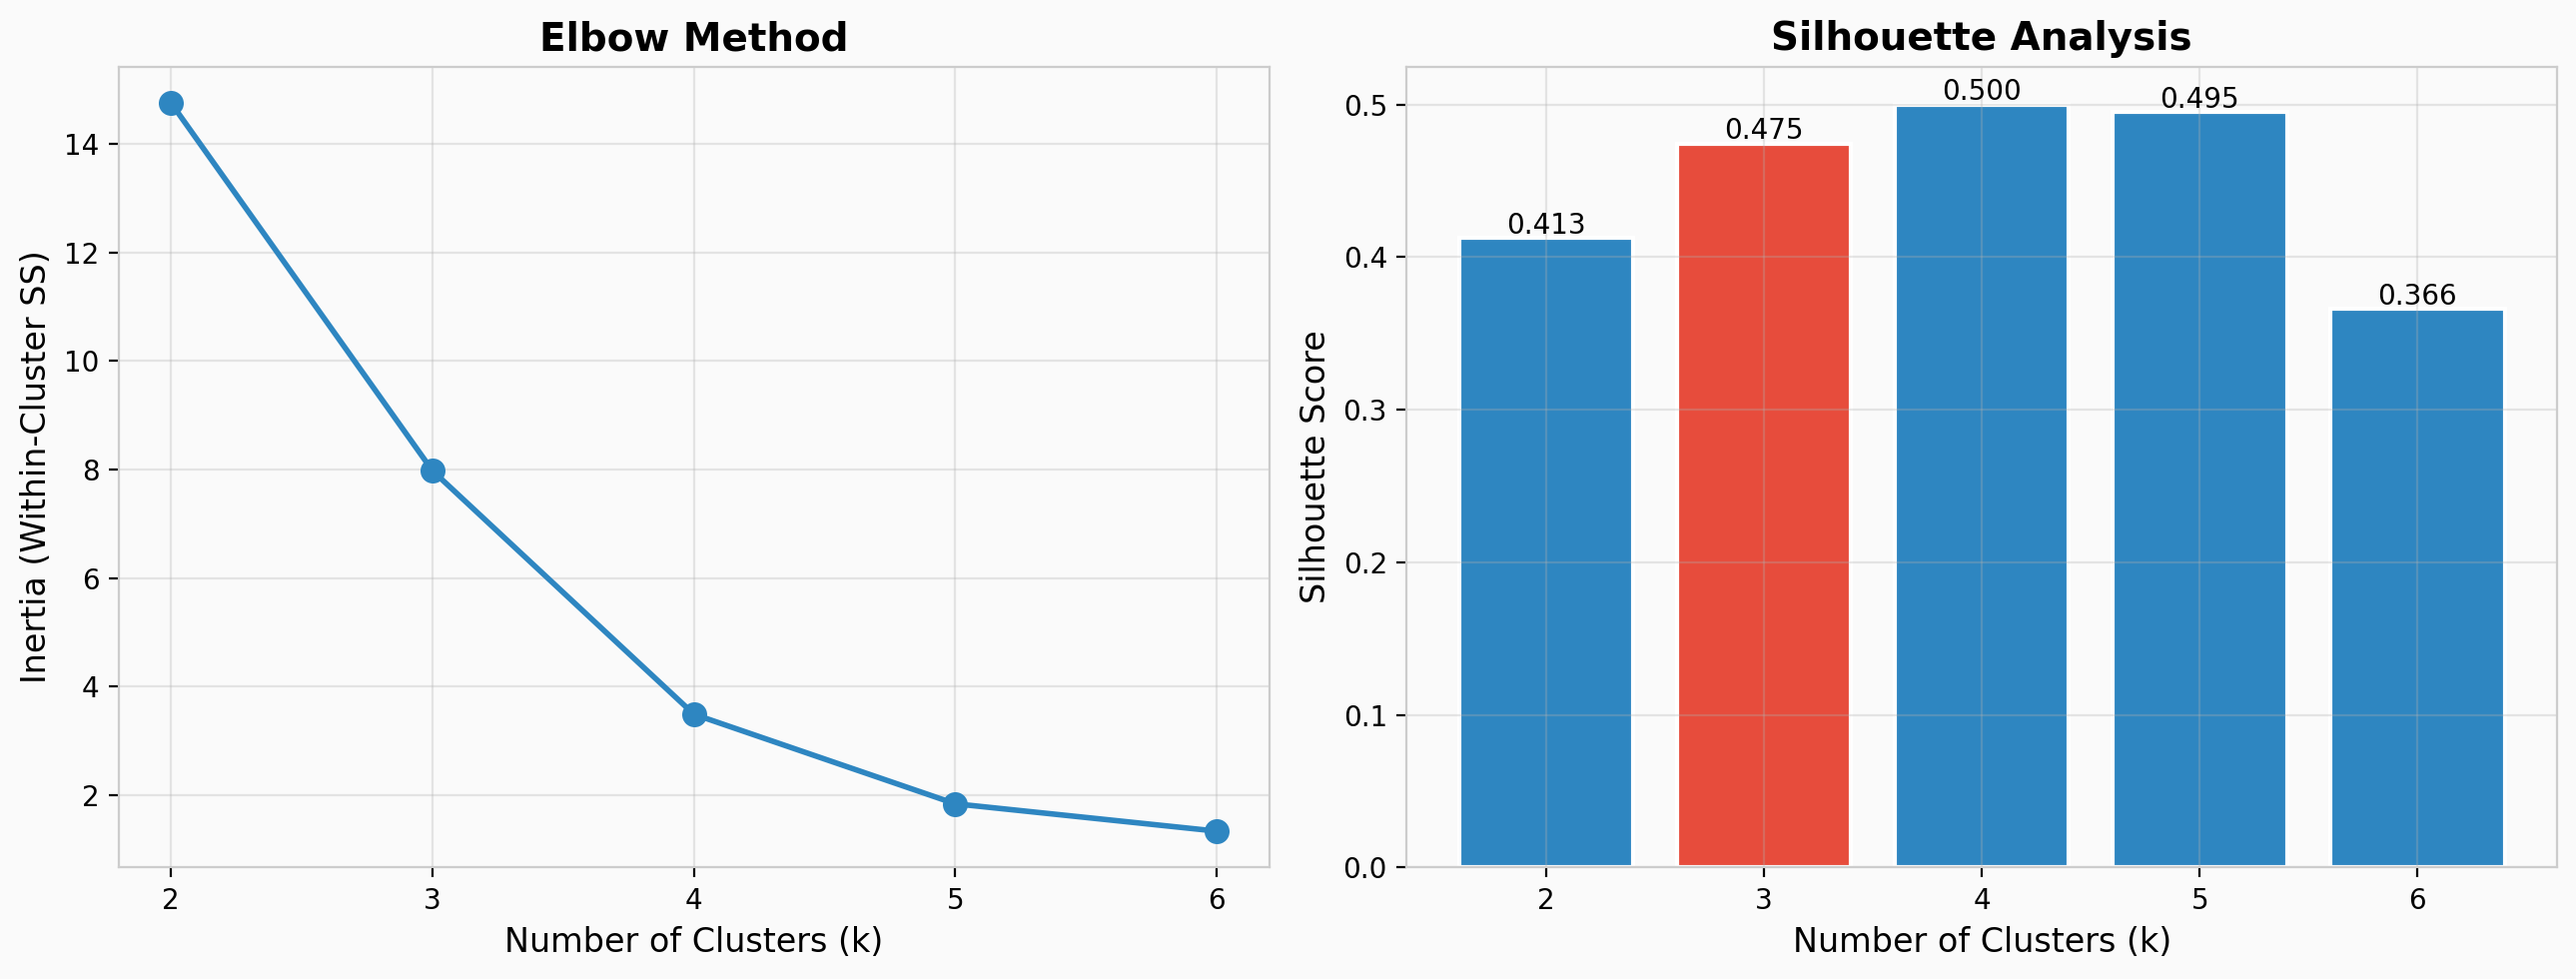
\includegraphics[width=\textwidth]{figures/01_k_selection.png}
\caption{Elbow plot (left) and silhouette scores (right) for $k = 2 \ldots 6$
on the filtered sample ($N = 10$).}
\end{figure}

\begin{table}[H]
\centering
\begin{tabular}{@{}clccc@{}}
\toprule
\textbf{Cluster} & \textbf{Persona} & \texttt{dospert\_fin} & \texttt{rng\_pumps} & \texttt{impulsivity} \\
\midrule
C0 & Consistent Conservatives   & z $= -1.10$ & z $= -1.03$ & z $= +0.40$ \\
C1 & Deliberate Risk-Takers     & z $= +0.38$ & z $= +0.97$ & z $= -1.02$ \\
C2 & Impulsive Risk-Seekers     & z $= +0.60$ & $\approx 0$ & z $= +0.96$ \\
\bottomrule
\end{tabular}
\caption{Z-scored cluster profiles at $k = 3$ ($N = 10$, silhouette $= 0.475$).}
\end{table}

\begin{figure}[H]
\centering
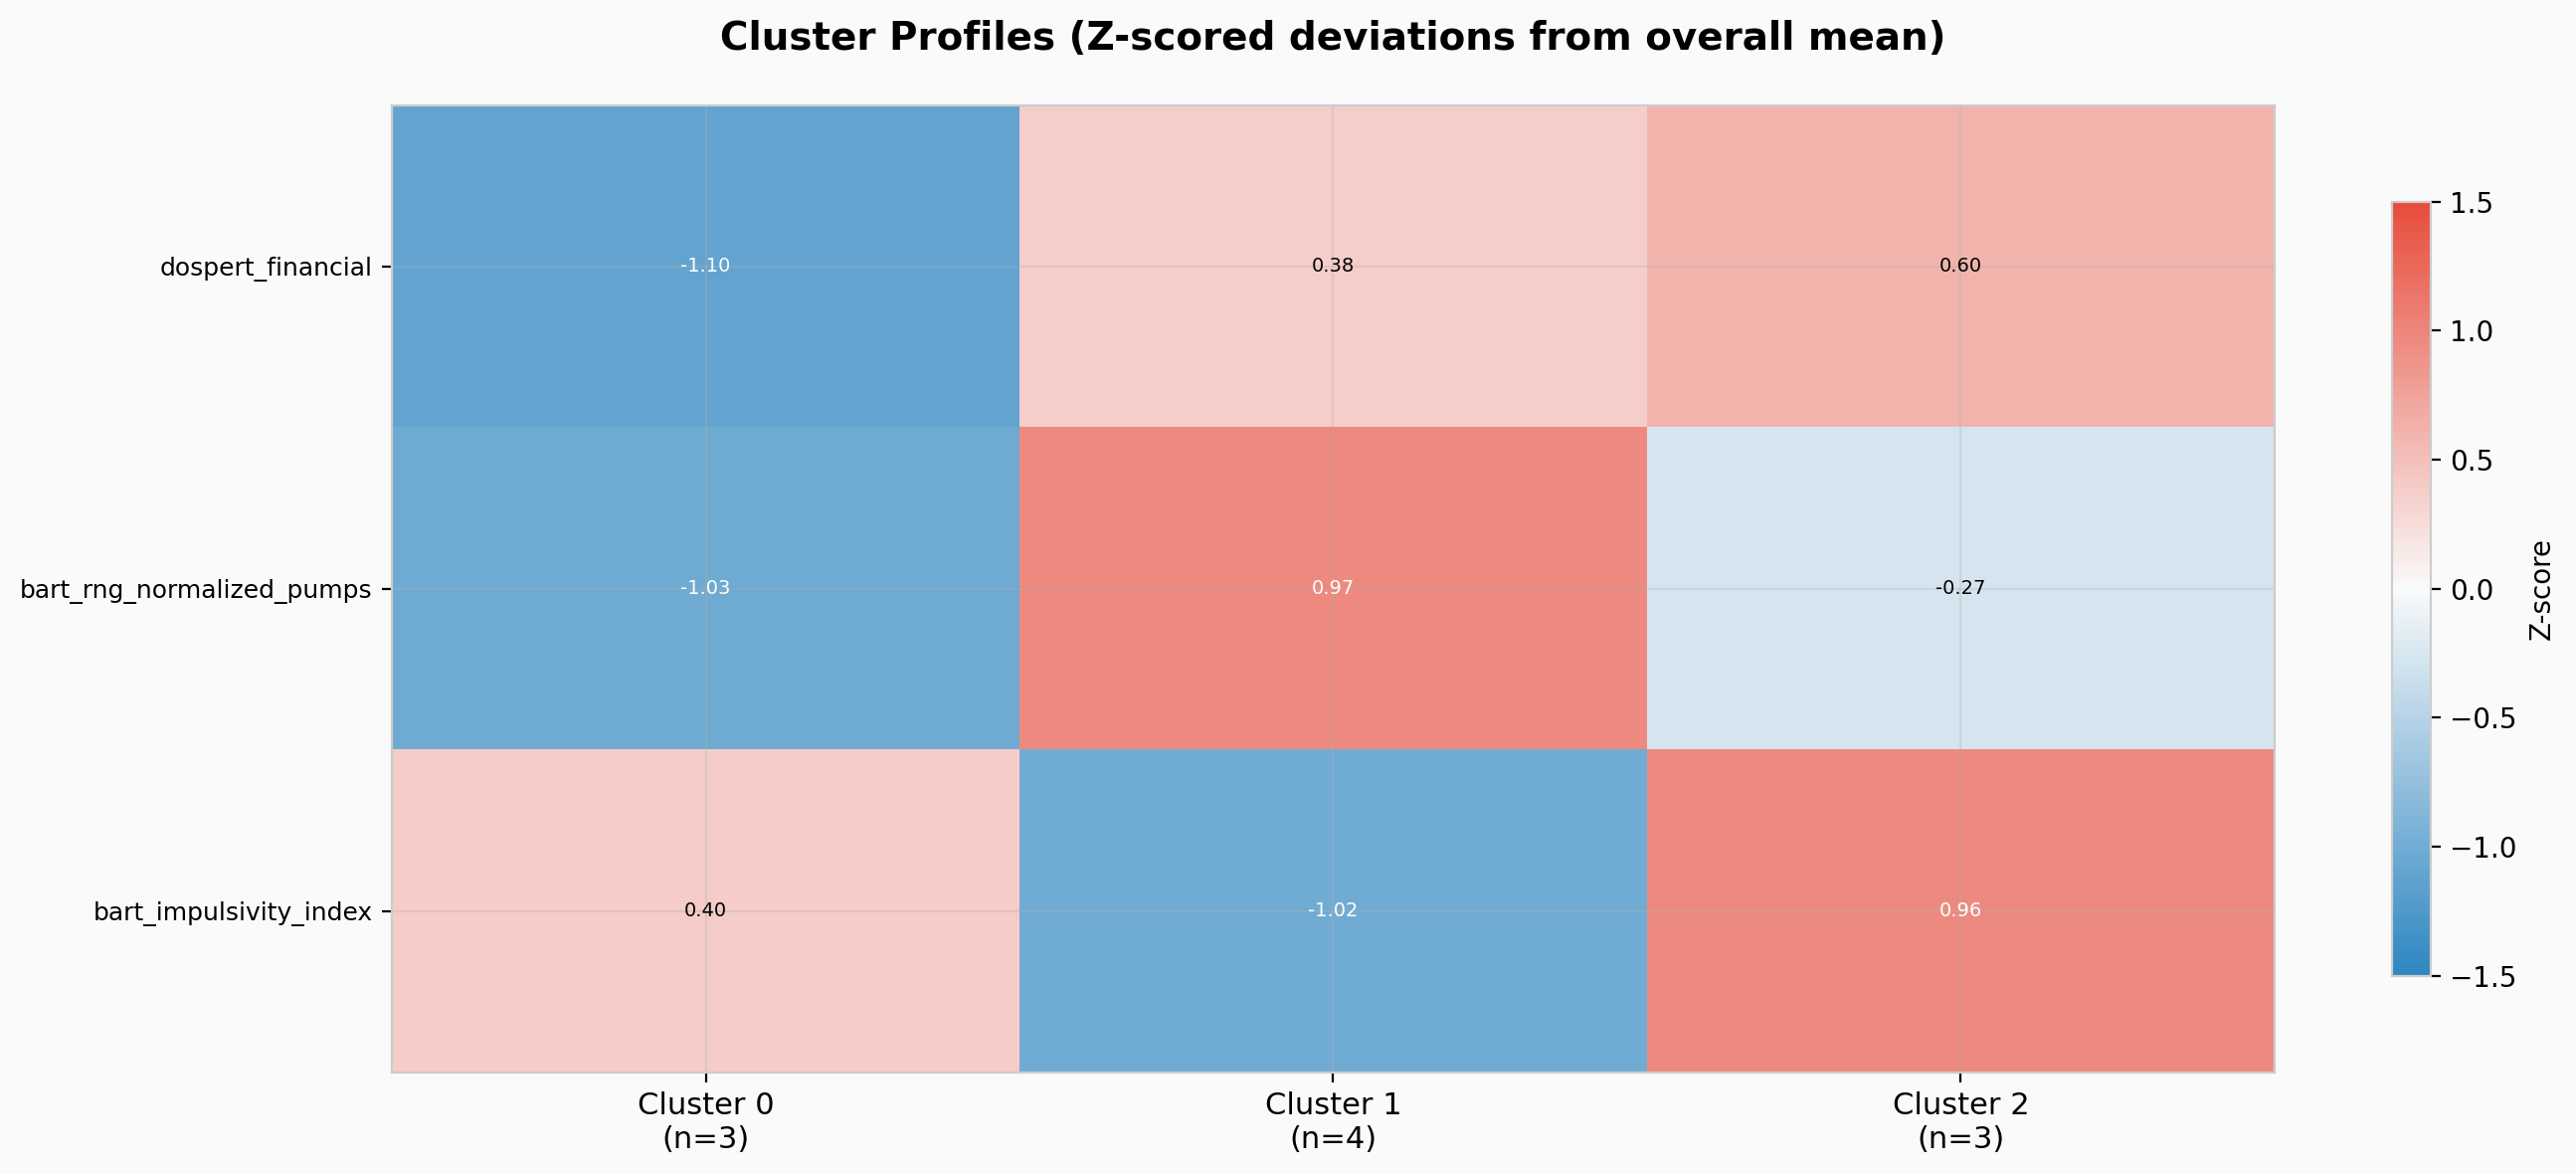
\includegraphics[width=\textwidth]{figures/02_cluster_profiles.png}
\caption{Z-scored cluster centroids ($N = 10$, prior task excluded).}
\end{figure}

\textbf{C0 --- Consistent Conservatives} ($n = 3$). Low self-reported
financial risk tolerance and low behavioral risk on BART. The mild
impulsivity uptick suggests that when they do pump, they are not
particularly strategic about it --- conservative by conviction, not by
calculation.

\textbf{C1 --- Deliberate Risk-Takers} ($n = 4$). Push close to balloon
limits (high normalized pumps) with low impulsivity --- slow, consistent
timing and controlled explosion rates. Their self-report is only
moderately above average, suggesting they may not perceive their own
behavior as particularly risky.

\textbf{C2 --- Impulsive Risk-Seekers} ($n = 3$). Report the highest
financial risk tolerance and act on it impulsively --- fast clicking,
excess explosions. Their normalized pumps are near zero because they
blow up before reaching their intended targets. They \emph{intend} to
take risks but their approach is reactive, not strategic.

The headline: C1 and C2 both report above-average financial risk appetite,
but BART reveals fundamentally different strategies. Self-report alone
cannot distinguish deliberate from impulsive risk-taking.

\subsection{PCA}

\begin{figure}[H]
\centering

\includegraphics[width=0.85\textwidth]{figures/03_pca_projection.png}
\caption{PCA projection ($N = 10$). PC1 separates deliberate risk-takers
(C1) from the rest along the behavioral axis. PC2 is almost entirely
\texttt{dospert\_financial} (loading $= 0.821$).}
\end{figure}

PC1 ($\sim$50\%) separates C1 from the rest along the
\texttt{rng\_normalized\_pumps} vs.\@ \texttt{impulsivity\_index} axis.
PC2 ($\sim$37\%) is dominated by \texttt{dospert\_financial} (loading $= 0.821$),
meaning the self-report and behavioral dimensions are close to orthogonal.
People who \emph{say} they take financial risks and people who
\emph{actually} take them on BART are not necessarily the same --- which
is the core convergent validity finding.


% ──────────────────────────────────────────────────────────────────────────
\section{Summary of Changes}
% ──────────────────────────────────────────────────────────────────────────

\begin{table}[H]
\centering\small
\begin{tabular}{@{}lll@{}}
\toprule
\textbf{Metric} & \textbf{Before (v1)} & \textbf{After (v2)} \\
\midrule
Risk calibration    & \texttt{risk\_adjustment\_score} (linear distance) & \texttt{ev\_ratio\_score} (EV-weighted) \\
Color discrimination & \texttt{color\_discrimination\_index} (Cohen's $d$) & \texttt{ev\_efficiency\_differentiation} ($1 - \text{CV}$) \\
Impulsivity         & Orange pumps / 8 (often missing) & Composite: timing + explosions + orange \\
Explosion penalty   & --- & New: excess over EV-optimal baseline \\
Risk calibration    & --- & New: EV-ratio $\times$ (1 $-$ penalty) \\
Flat strategy       & --- & New: boolean detection flag \\
Between-balloon CV  & Global CV across all colors & Per-color CV, then averaged \\
Adaptive strategy   & Equal 33/33/33 weighting & Conditional + 10\% money efficiency \\
Money efficiency    & --- & New: realized earnings / EV-optimal expected \\
Clustering          & 5 features, $N=15$, $k=2$ & 3 features, $N=10$ (prior task excluded), $k=3$ \\
\bottomrule
\end{tabular}
\end{table}

None of the raw event collection, session validation, or per-color
segmentation logic has changed. The explosion model is the same sequential
Bernoulli. The DOSPERT scoring is unchanged. Everything upstream of the
scoring engine is identical to the previous version.

\end{document}
